\documentclass[11pt, letterpage]{article}
\usepackage[margin = 2cm]{geometry}
\usepackage{graphicx}
\usepackage[labelfont=bf, labelsep=period]{caption}
\RequirePackage{newfloat}
\DeclareFloatingEnvironment[fileext=los, listname=Lista de Esquemas, name=Esquema, placement=tbhp]{scheme}

\begin{document}
\begin{center}
	\huge
	\scshape Laboratorio Q. Avanzada \\
	\LARGE S\'intesis de Dilantin a partir de benzaldehido
	\\
	\normalsize
\end{center}

\section{Primera etapa}
\begin{scheme}
	\caption{Mecanismo de dimerizaci\'on del benzaldeh\'ido.}
	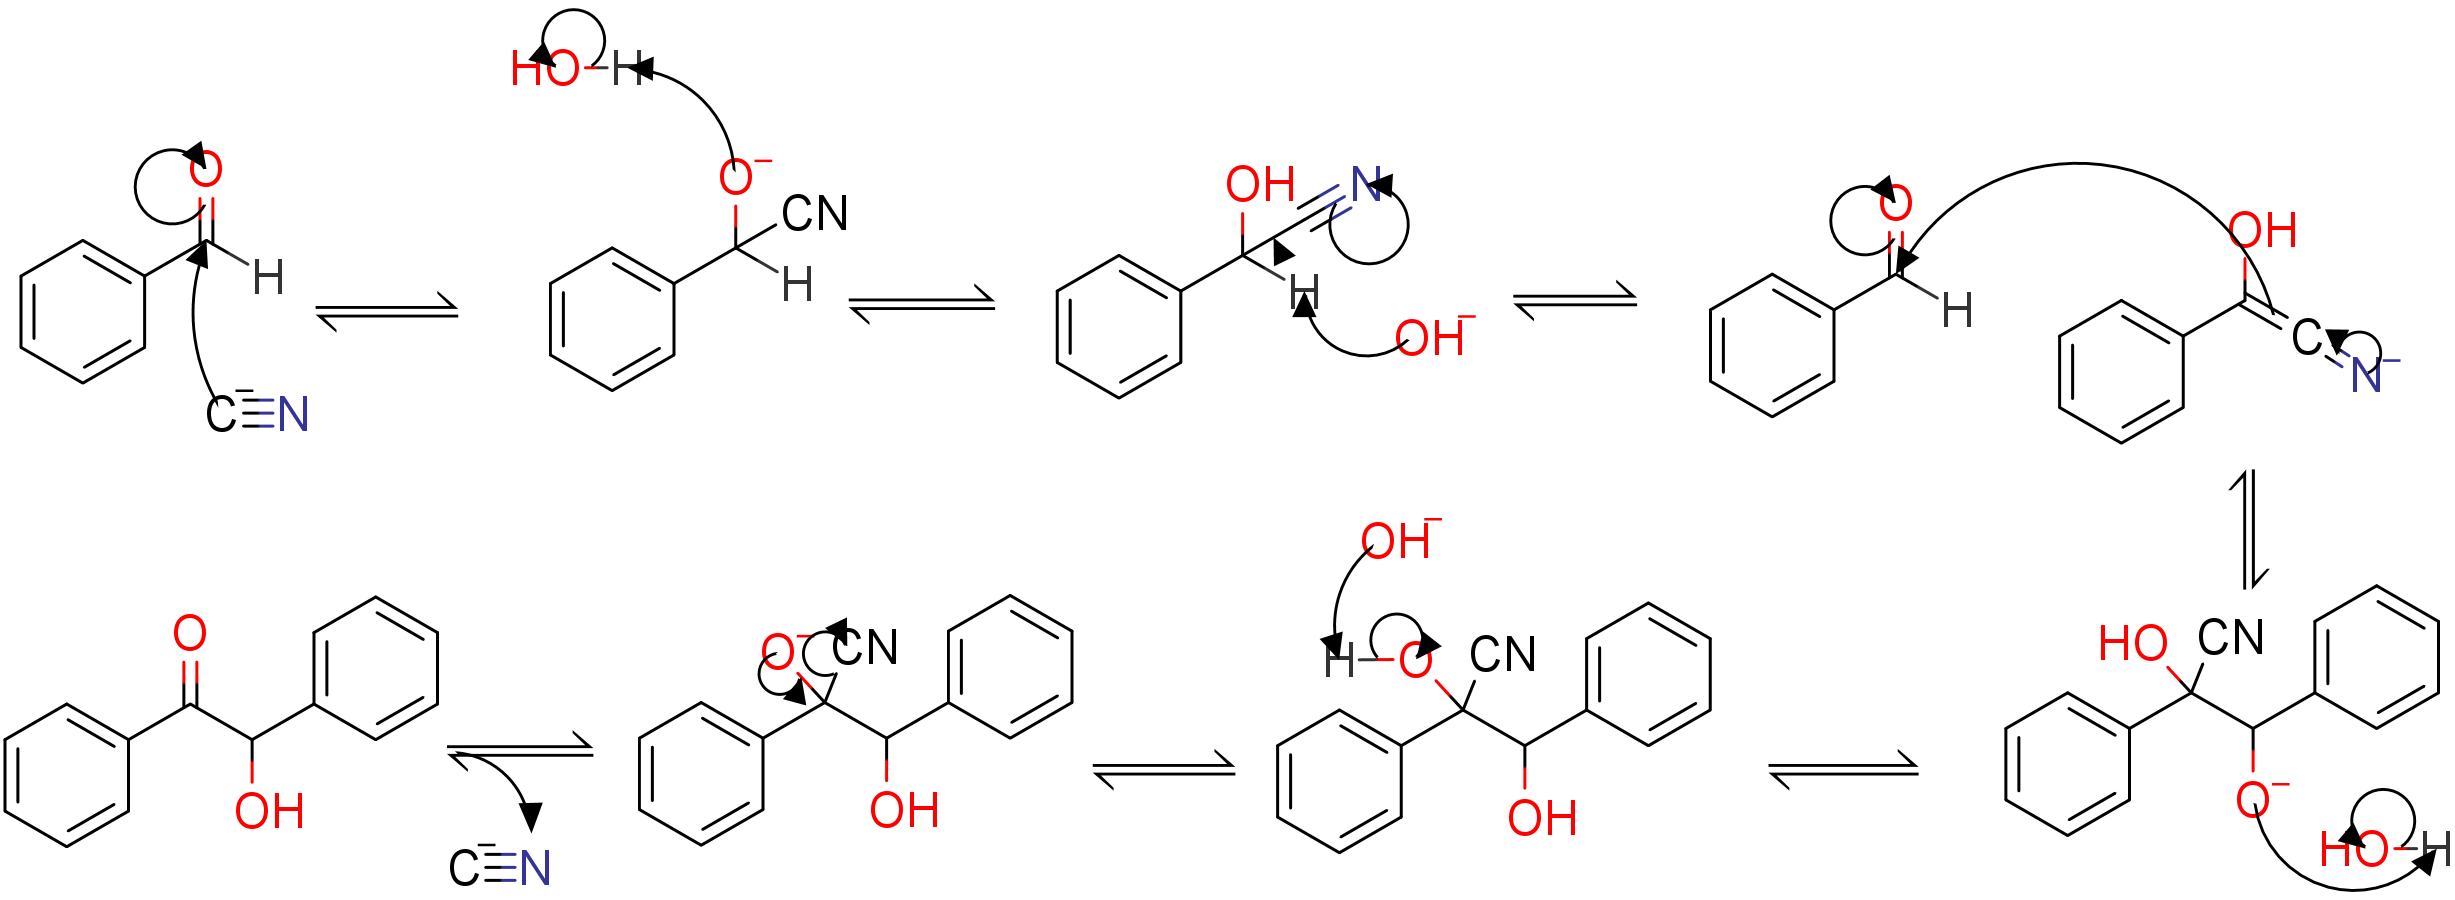
\includegraphics[width=\linewidth]{mechanism-condensacion.png}

\end{scheme}

\subsection{Procedimiento experimental}
\subsubsection{Destilar benzaldeh\'ido}
El benzaldeh\'ido se oxida con facilidad al \'acido benz\'oico, siendo este su contaminante m\'as frecuente. Es posible proteger al benzaldeh\'ido usando hidroquinona, la cual reacciona con el ox\'igeno circundante.
\subsubsection{Condensaci\'on benzo\'inica}
En un bal\'on de 50 mL disolver 5.0 mL (47 mmol) de benzaldehido previamente destilado en 6.5 mL de etanol al 95 \%; a esta mezcla adicione una soluci\'on de 500 mg de cianuro de sodio en 5.0 mL de agua. Caliente la mezcla a reflujo constante durante 30 minutos. Seguido este tiempo retire el calentamiento y observe la soluci\'on. Deber\'ian formarse cristales al cabo de unos minutos, si no observa el cambio lleve el bal\'on a un ba\~no de hielo y enfr\'ielo hasta que vea los cristales. F\'iltrelos y l\'avelos con agua fr\'ia. La benzoina cruda debe ser de un color blanco o p\'alidamente amarillo. El rendimiento de la reacci\'on es cercano al 90 \% \cite{Benzoin}. 

La sustancia pura se obtiene por recristalizaci\'on usando etanol al 95 \%, la relaci\'on sustrato/solvente es 0.13 g/mL. La benzoina se disuelve en alcohol en ebullici\'on cerca de 8 \% se pierde con la purificaci\'on. La cantidad de benzoina final debe ser cercana a 8.2 g \cite{Benzoin}.

\bibliographystyle{unsrt}
\begin{thebibliography}{9}
	\bibitem{Benzoin}
	\textit{Organic Syntheses} 1921, 1, 33
\end{thebibliography}

\newpage
\section{Segunda etapa}
\begin{scheme}[h]
	\centering
	\caption{Oxidaci\'on de la benzoina en presencia de \'acido n\'itrico.}
	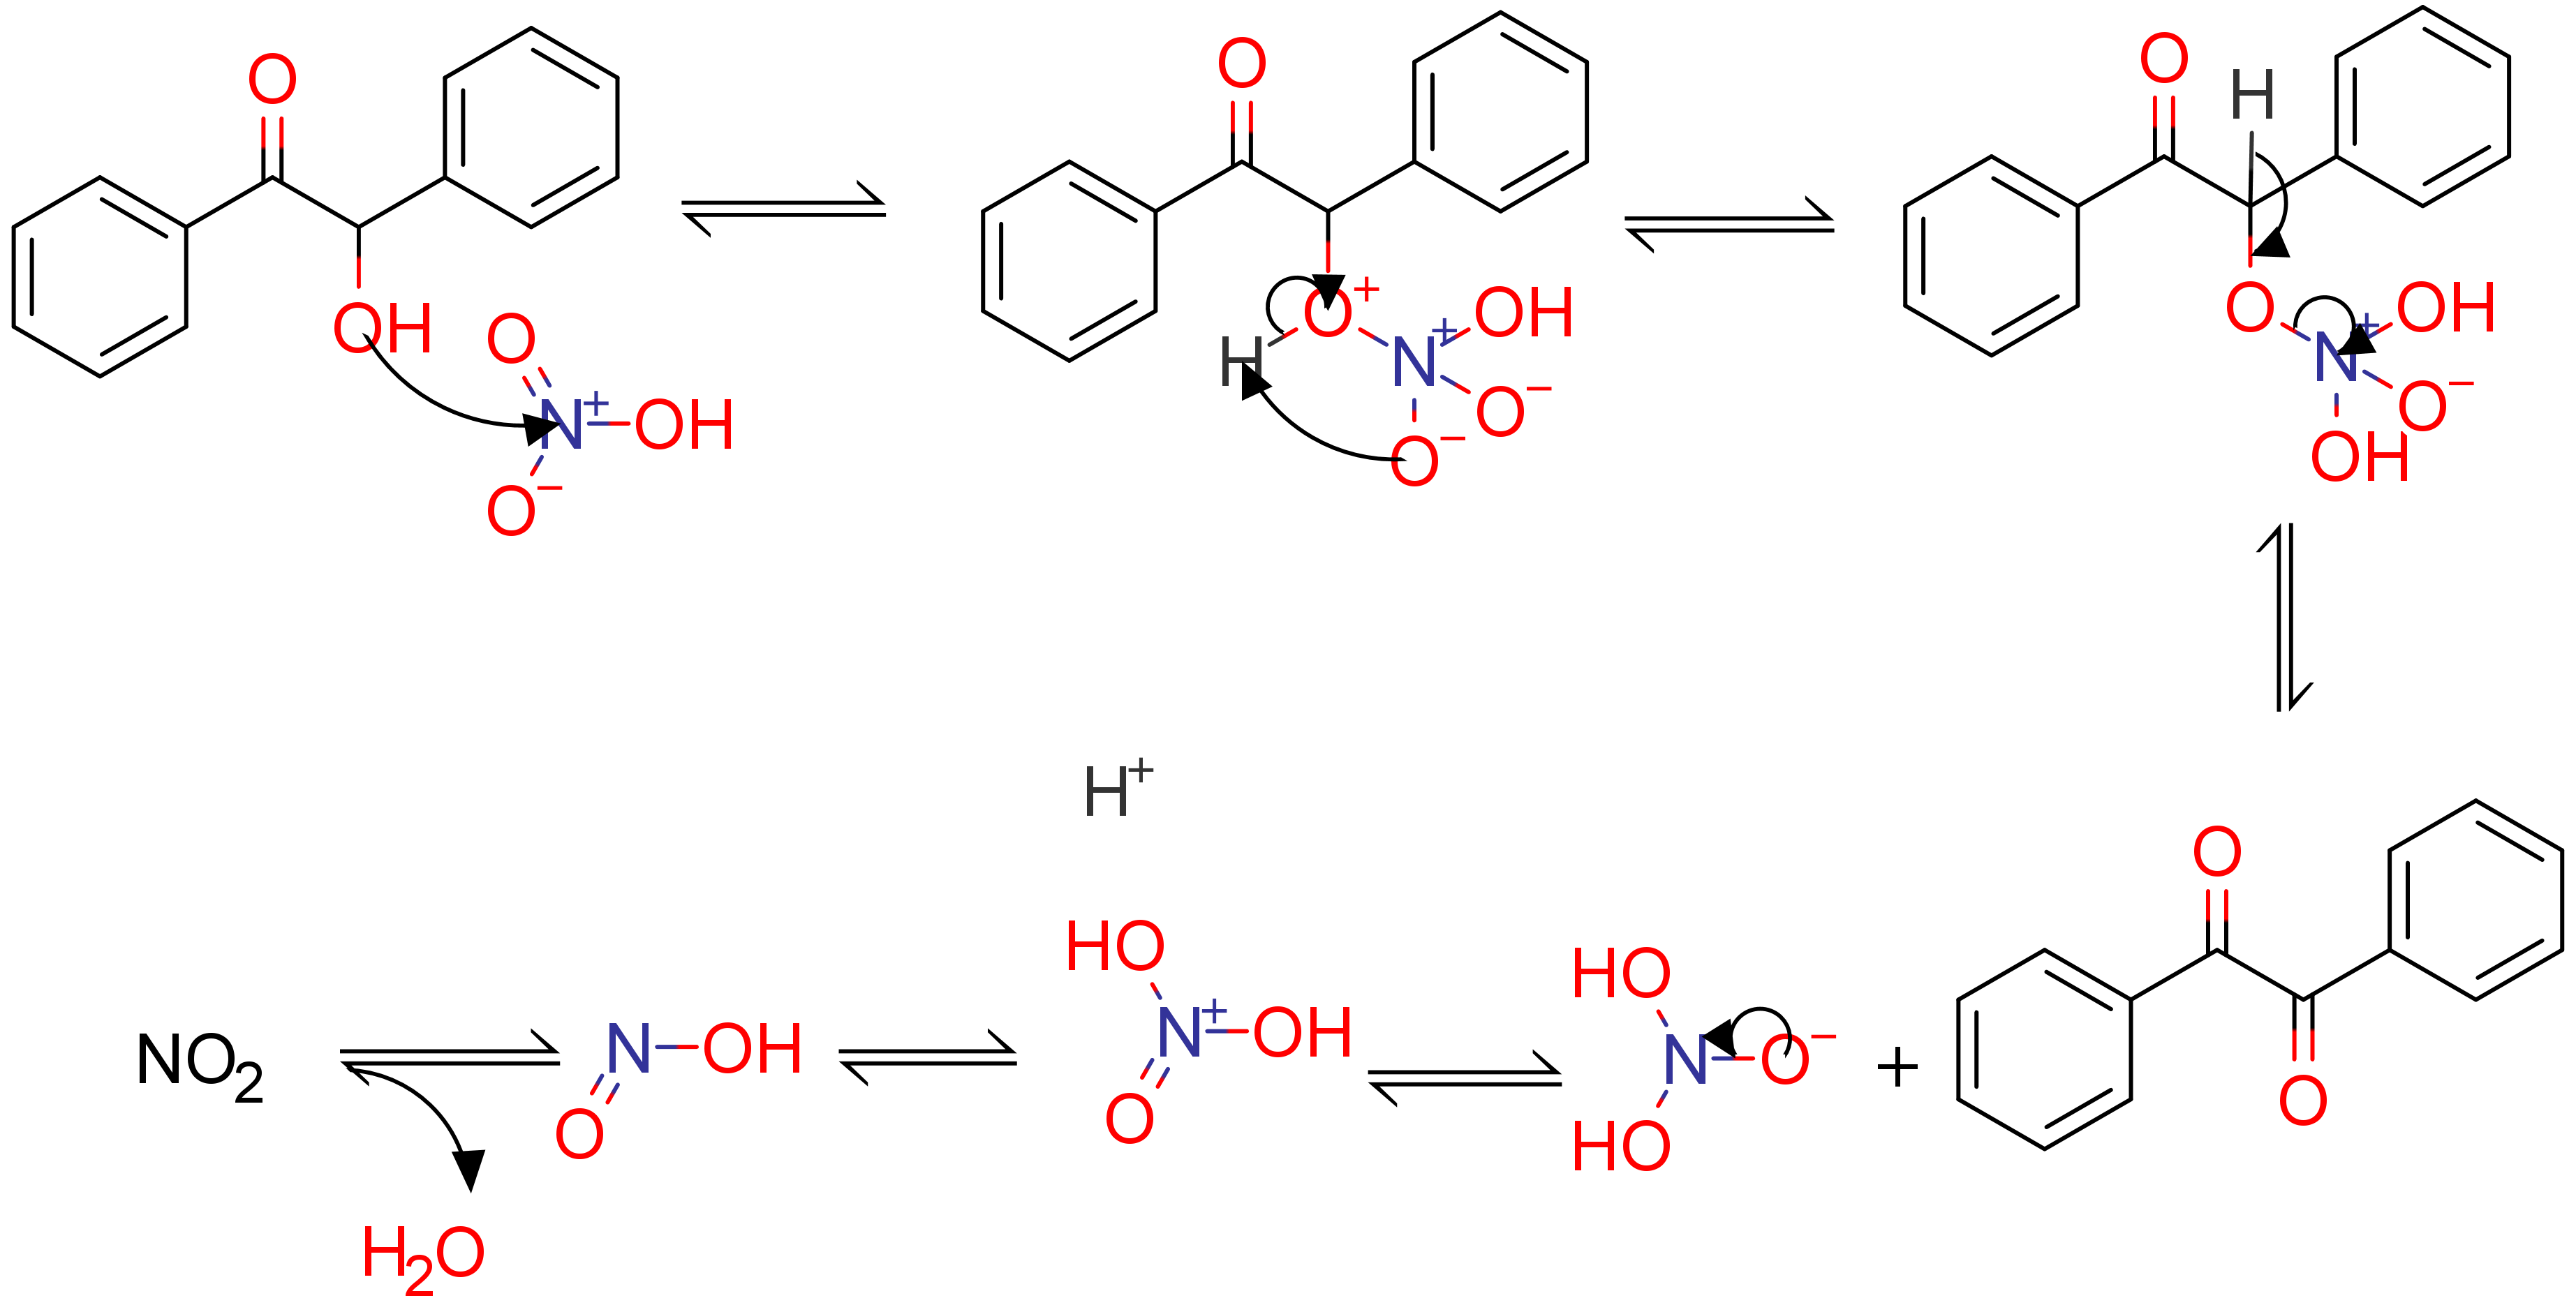
\includegraphics[width=0.8\linewidth]{mechanism-oxidation.png}
\end{scheme}

\newpage
\section{Tercera etapa}
\begin{scheme}
	\centering
	\caption{Formaci\'on}
	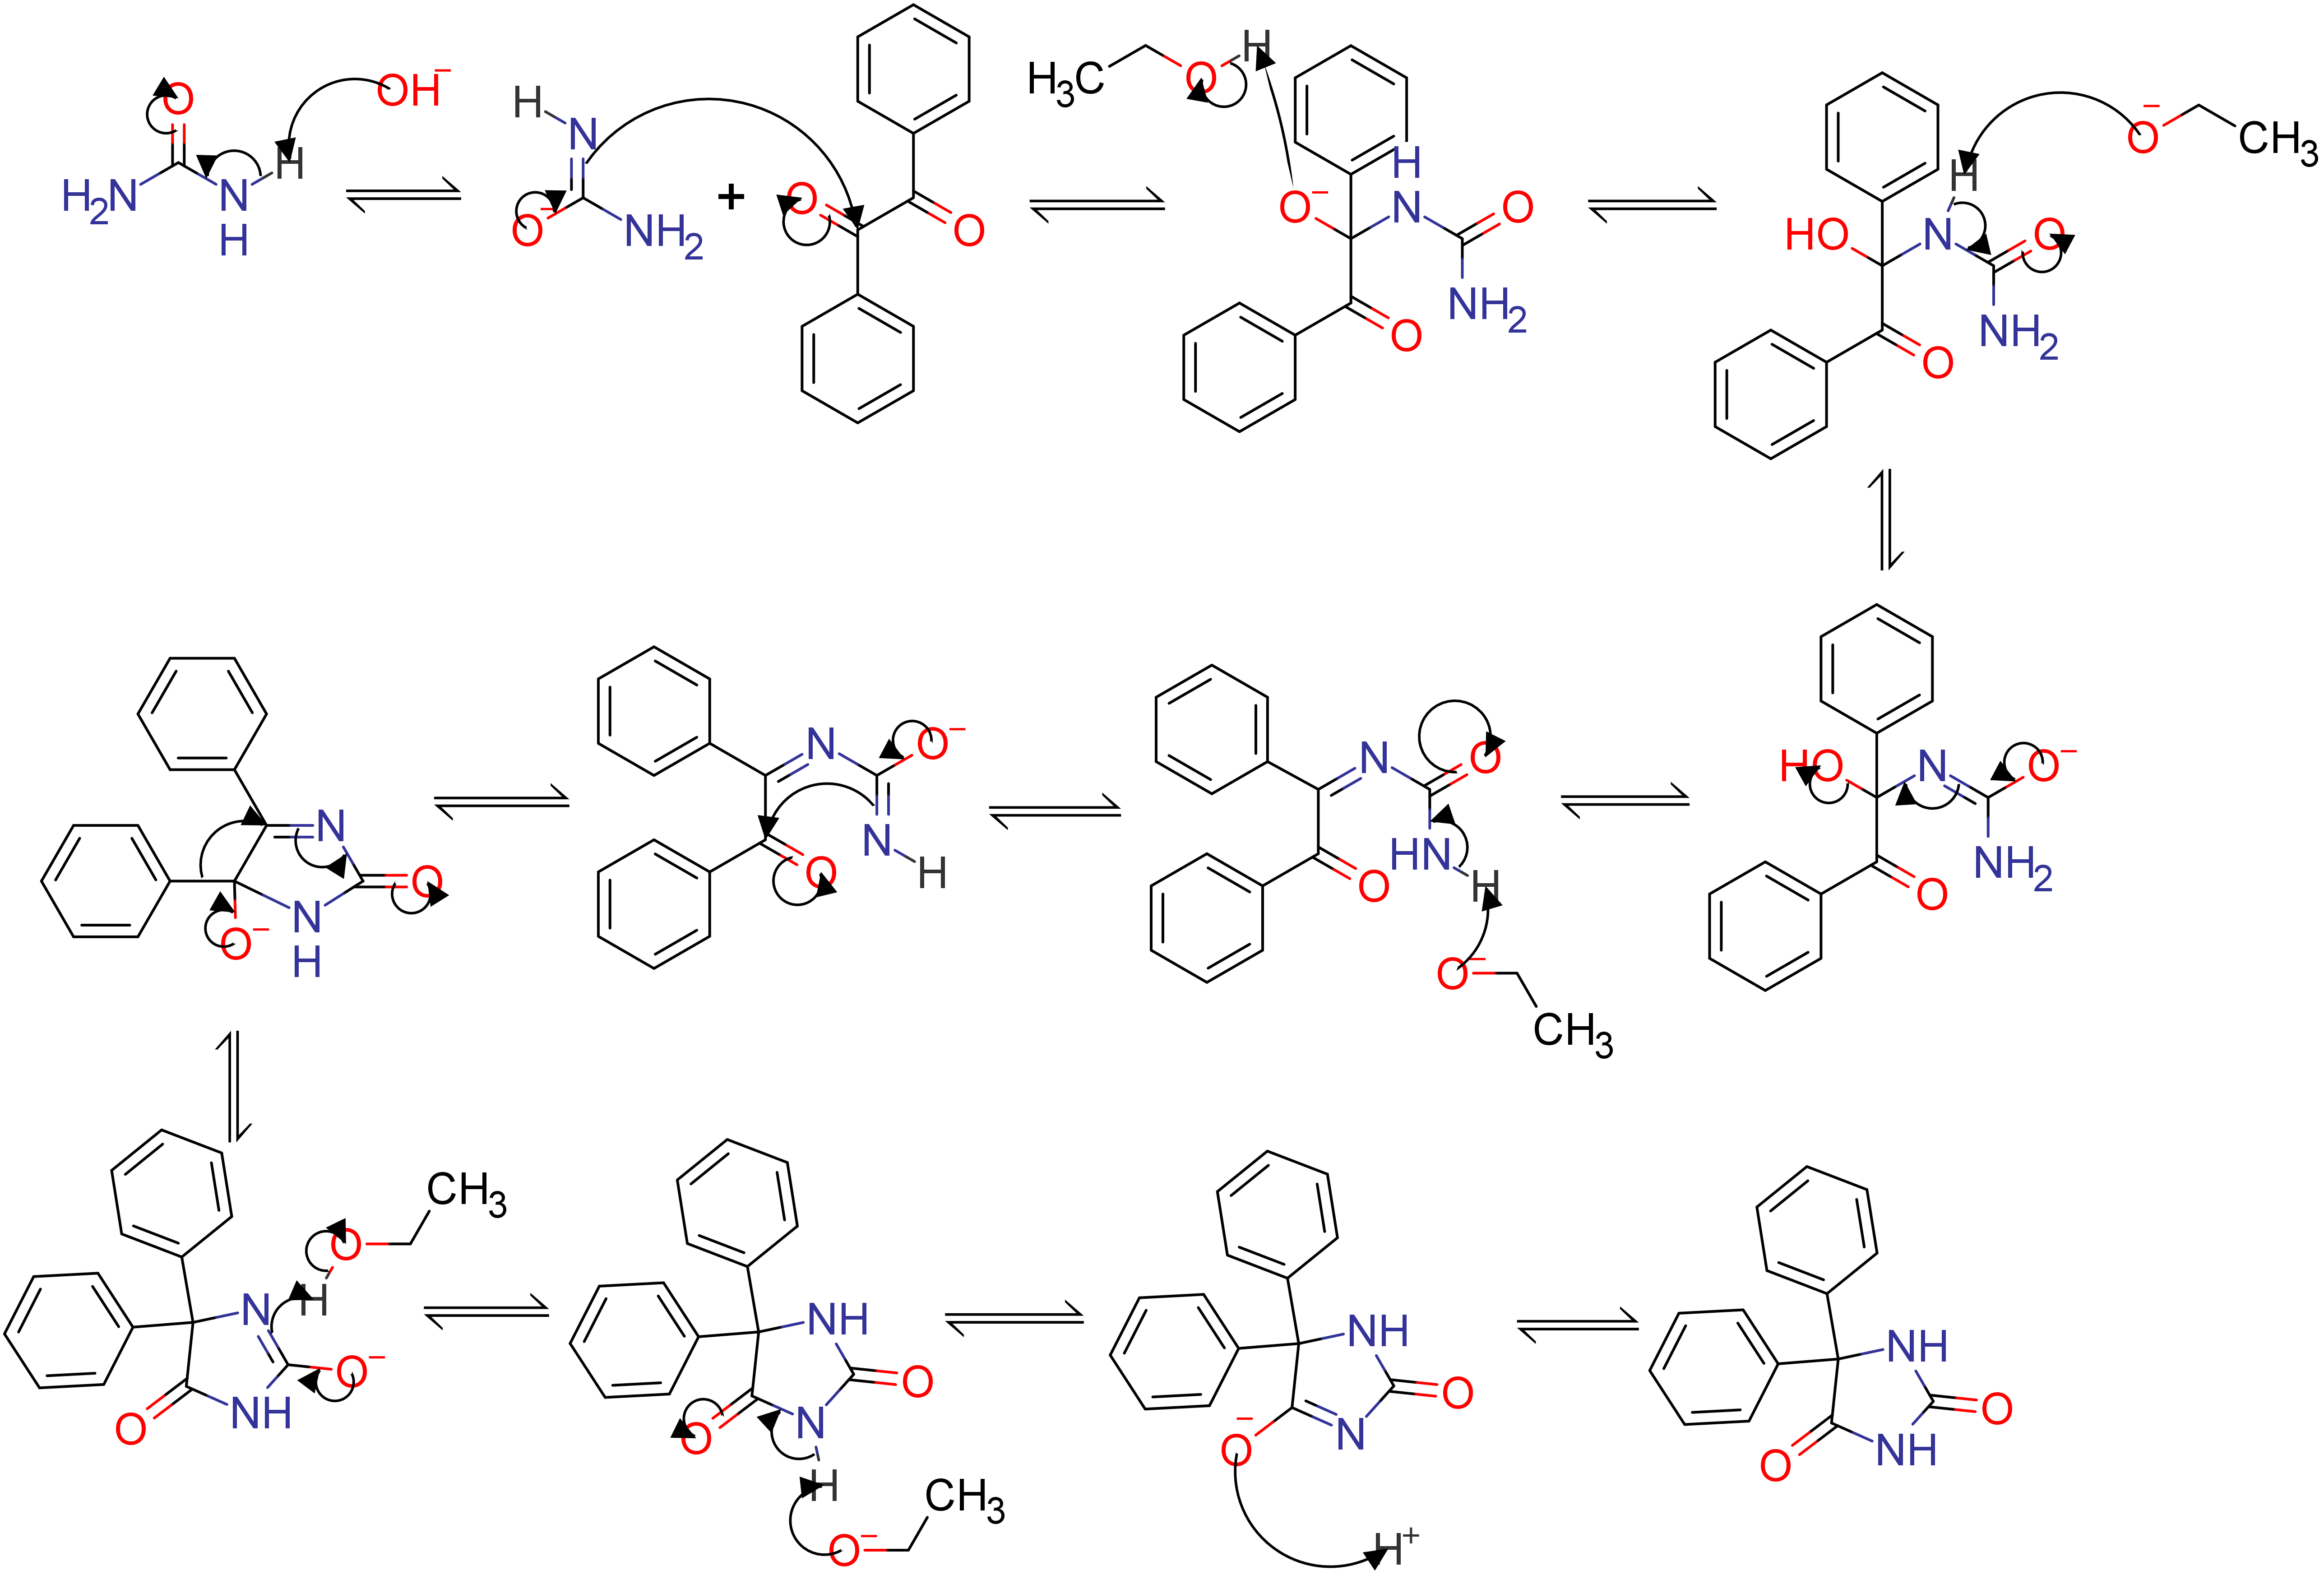
\includegraphics[width=\linewidth]{mechanism-formation.png}
\end{scheme}

\small
\verb|http://www.umich.edu/~chem216/216%20S11-Expt%205.pdf|

\verb|http://www.academicjournals.org/article/article1379423378_Gbaguidi%20et%20al.pdf|

\verb|http://organicsynthesisinternational.blogspot.com.co/2014/12/dilantin-55-diphenylhydantoin.html|

\end{document}
